\documentclass[9pt]{IEEEtran}

\usepackage[english]{babel}
\usepackage{graphicx}
\usepackage{epstopdf}
\usepackage{fancyhdr}
\usepackage{amsmath}
\usepackage{amsthm}
\usepackage{amssymb}
\usepackage{url}
\usepackage{array}
\usepackage{textcomp}
\usepackage{listings}
\usepackage{hyperref}
\usepackage{xcolor}
\usepackage{colortbl}
\usepackage{float}
\usepackage{gensymb}
\usepackage{longtable}
\usepackage{supertabular}
\usepackage{multicol}

\usepackage[utf8x]{inputenc}

\usepackage[T1]{fontenc}
\usepackage{lmodern}{}
\input{glyphtounicode}
\pdfgentounicode=1

\graphicspath{{./figures/}}
\DeclareGraphicsExtensions{.pdf,.png,.jpg,.eps}

% correct bad hyphenation here
\hyphenation{op-tical net-works semi-conduc-tor trig-gs}

% ============================================================================================

\title{\vspace{0ex}
MCMC homework}

\author{Marko Medved\vspace{-4.0ex}}

% ============================================================================================

\begin{document}

\maketitle

 \section{Numerical integration vs Monte Carlo integration}
 In this section we compare numerical integration to Monte Carlo integration 
 on a simple domain where the standard numerical integration is possible. Concretly, we approximate 
 the expected value of the (a, b, c)-PERT distribution:

\[
p(x) = \frac{(x - a)^{\alpha - 1} \cdot (c - x)^{\beta - 1}}{\mathrm{B}(\alpha, \beta) \cdot (c - a)^{\alpha + \beta - 1}}
\]
 with a = 0, b = 10 and c = 100. 


 \subsection{Trapezoidal rule}
We begin by approximating the expected value using the Trapezoidal rule.
 To determine how many function evaluations are required, we first
  computed the exact expected value analytically: 
  $\mathbb{E}[X] = 23.\overline{3}$. We then applied the numerical method,
   incrementally increasing the number of function evaluations until the
    result was accurate to four decimal places (the difference between estimated 
    and true value was less that $5 \times 10^{-5}$). This level of precision was 
    achieved with 271 evaluations.

 \subsection{CLT estimation for Monte-Carlo}
In this section, we estimate the expected value using Monte Carlo integration.
 Our objective is to determine how many random samples are needed to approximate
  the integral within two decimal places, with 95\% confidence.
 
The Monte-Carlo approximation in this example is done by drawing
 independent samples
  \( x_1, x_2, \dots, x_n \sim \mathcal{U}(a, c) = \mathcal{U}(0, 100) \), and estimating:

\[
\mathbb{E}[X] = \int_a^c x \cdot p(x) \, dx \approx \frac{c - a}{n} \sum_{i=1}^n x_i p(x_i).
\]

Let this estimator be denoted by \( \hat{\mu}_n \). By the Central Limit Theorem, the standard error of \( \hat{\mu}_n \) is approximately:

\[
SE = \frac{\hat{\sigma}}{\sqrt{n}},
\]

where \( \hat{\sigma}^2 \) is the sample variance of the integrand values \( x_i p(x_i) \).

To estimate \( \mathbb{E}[X] \) to 2 decimal places with 95\% confidence, we require:

\[
1.96 \cdot \frac{\hat{\sigma}}{\sqrt{n}} \leq 0.005.
\]

So to estimate the number of points, we need to compute $\sigma$. Since this 
is the variance of our integrand, we decided to estimate it using a pilot run
 of $10^8$ samples. Our estimation was $\hat{\sigma} = 19.08$ and then we calculated: 
 $n \approx 55935632$. 



 \subsection{Numerical samples verification}
To verify our estimate of the required number of samples, we perform 
200 independent Monte Carlo simulations. We then compute the difference 
between each estimate and the true expected value, and visualize
 the distribution of these differences as a density plot in 
 Figure~\ref{fig:diff}. We can see that almost all samples, as expected since we defined the 
 95\% confidence, have an absolute 
 difference to the true value less than 0.005. We can also seee that the density is gathered 
 around 0. 

    \begin{figure}[h]
        \centering
        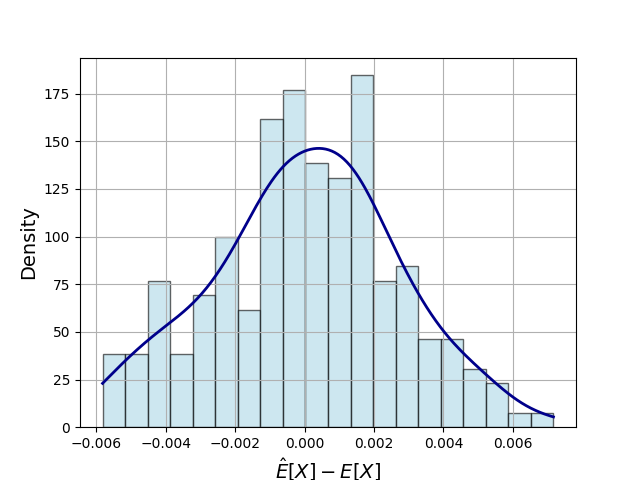
\includegraphics[width=0.99\columnwidth]{figures/diff.png}
        \caption{Density of differences of the estimated and true expected value}
        \label{fig:diff}
    \end{figure}



 \subsection{Comparison of results from both methods}
As expected, the trapezoidal rule significantly outperformed the Monte Carlo
 method. It provided a deterministic result accurate to four decimal places 
 using relatively few evaluations, while the Monte Carlo estimate required 
 many more samples and achieved only two-decimal-place accuracy with 95\%
  confidence. This highlights that for low-dimensional problems with simple
   domains, standard numerical integration methods are preferable to Monte 
   Carlo methods.

\section{Importance sampling}
In this section we implement importance sampling for Monte Carlo integration
 to be able to compute the provided integral:
 $I = \int_0^1 x^{-3/4} \cdot e^{-x} \, dx$.

We plot the integrand ($f(x) = x^{-3/4} \cdot e^{-x}$) on Figure\ref{fig:lin}. We can see that 
the bulk of the integral is gathered really close to 0.


    \begin{figure}[h]
        \centering
        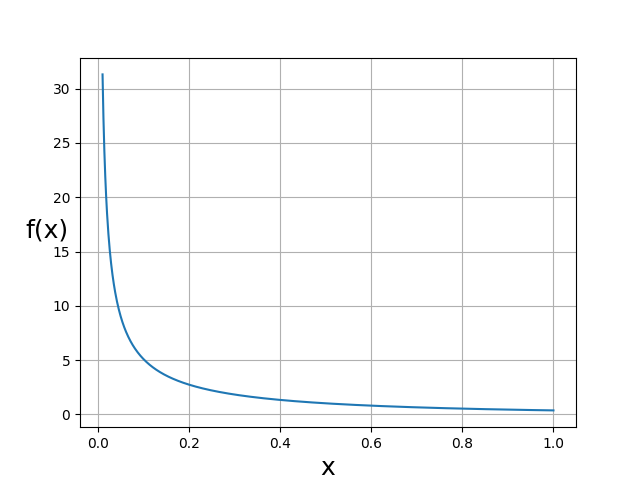
\includegraphics[width=0.99\columnwidth]{figures/f}
        \caption{Graph of the given integrand}
        \label{fig:lin}
    \end{figure}

 \subsection{Sampling from the Uniform distribution}
 Here we use the uniform distribution as the distribution we want to sample from.
 Since our uniform distribution is from 0 to 1, the estimation of the integral is
 simply: 
 \[
I \approx \frac{1}{n} \sum_{i=1}^{n} f(x_i)
\]
As we have seen on Figure~\ref{fig:lin}, the function has a shape that is very concentrated at 
0 so the uniform choice might not be the best. 

 \subsection{Sampling from the provided distribution}
 Next we use the provided distribution ($q(x) = c \times x^{-3/4}$).
 
 Firstly, we determine the $c$ constant to be $1/4$ so that the distribution
  integrates to 1 over the domain $[0, 1]$. 

 Next, to implement inversion sampling, we need the CDF and it's inverse. 
 We calculated these functions to be: 
\begin{align*}
F(x) &= x^{1/4} \\
F^{-1}(x) &= x^4
\end{align*}
Then we simply sampled from the uniform distribution on the $[0, 1]$ interval, 
and transformed those samples with our inverse CDF to get the samples of $q(x)$.

Lastly, we implemented the importance sampling. Our integral can now be approximated as:
\[
I \approx \frac{1}{n} \sum_{i=1}^{n} \frac{f(x_i)}{ q(x_i)}
\] 


 \subsection{Comparison of results from both methods}
Here we compare the results of two Monte Carlo integration methods. For each method, we drew 10 independent 
samples of size $n = 10^7$, computed the average estimate, and calculated the corresponding
 standard deviation. The results are summarized in Table~\ref{tab:imp}.  

\begin{table}[h]
    \centering
    \begin{tabular}{c|c|c}

    \textbf{Sampling Distribution} & \textbf{Estimate} & \textbf{Standard Deviation} \\
    \hline
    Uniform  & 3.3640 & 0.0890 \\
    $q(x)$ & 3.3795 & 0.0001 \\
    \end{tabular}
    \caption{Comparison of Importance Sampling Estimates}
    \label{tab:imp}
\end{table}

As shown in the table, using $q(x)$ as a proposal distribution results in a significantly 
lower standard deviation compared to uniform sampling. This improvement is expected, as
$q(x)$ closely matches the shape of the integrand, leading to more samples being drawn
 from regions that contribute most to the integral. Consequently, the variance of the 
 estimator is greatly reduced.

\section{Metropolis-Hastings algorithm}
Here, we implement the Metropolis-Hastings (MH) algorithm to estimate the mean and variance of the parameters \(\alpha\) and \(\eta\) of the Weibull distribution, which models our random variable.


Firstly, we compute the posterior from the given likelihood and prior: 
\[
p(\alpha, \eta | x) \propto \left( \prod_{i=1}^{n} \alpha \, \eta \, x_i^{\alpha - 1} \, e^{-\eta x_i^\alpha} \right) \cdot e^{-\alpha - 2 \eta} \, \eta
\]

Note that we use the data provided in the instructions. Note also that for 
all of the constructed chains we use the initial point of $[1, 1]$.

\subsection{Multivariate normal proposal}
To sample from the posterior distribution 
\[
p(\alpha, \eta \mid \vec{x}),
\]
we firstly implemented the algorithm using a multivariate normal proposal distribution.

We tested several covariance matrices
by running 5 independent MH chains for each one.

For each setting, we computed the sum of effective sample sizes (ESS) across all chains
 for each parameter (\( \alpha \) and \( \eta \)).

\vspace{1em}

The following covariance matrices were selected for testing:


\begin{itemize}
  \item 
  \(
  \begin{bmatrix}
    0.1 & 0.0 \\
    0.0 & 0.1
  \end{bmatrix}
  \) 
  \hfill Small step sizes in both directions

  \item 
  \(
  \begin{bmatrix}
    1.0 & 0.0 \\
    0.0 & 1.0
  \end{bmatrix}
  \) 
  \hfill Large step sizes in both directions

  \item 
  \(
  \begin{bmatrix}
    0.5 & 0.01 \\
    0.01 & 0.5
  \end{bmatrix}
  \) 
  \hfill Moderate scale with weak correlation

  \item 
  \(
  \begin{bmatrix}
    0.5 & 0.05 \\
    0.05 & 0.5
  \end{bmatrix}
  \) 
  \hfill Moderate scale with stronger correlation

  \item 
  \(
  \begin{bmatrix}
    1.0 & 0.0 \\
    0.0 & 0.1
  \end{bmatrix}
  \) 
  \hfill Larger steps for \( \alpha \), smaller steps for \( \eta \)

  \item 
  \(
  \begin{bmatrix}
    0.1 & 0.0 \\
    0.0 & 1.0
  \end{bmatrix}
  \) 
  \hfill Smaller steps for \( \alpha \), larger steps for \( \eta \)
\end{itemize}

In Table~\ref{tab:ess_covariances}, we observe the effective sample sizes (ESS) obtained using different proposal covariance matrices. 

Larger step sizes generally produced better results, as evidenced by the higher ESS values for both $\alpha$ and $\eta$. Interestingly, the highest ESS for each individual parameter was achieved using imbalanced covariance matrices (the last two entries). Specifically, the matrix with a large variance for $\alpha$ and small for $\eta$ yielded the best ESS for $\alpha$, while the reverse configuration performed best for $\eta$.

However, the most balanced performance across both parameters was achieved when using a covariance matrix with large variances in both directions:
\[
\begin{bmatrix}
1.0 & 0.0 \\
0.0 & 1.0
\end{bmatrix}
\]
This choice provides a good trade-off, achieving high ESS for both parameters without favoring one over the other.
That is why this covariance matrix will be used for further evaluation. 

\begin{table}[H]
\centering
\renewcommand{\arraystretch}{1.4}
\begin{tabular}{c|c|c}

\textbf{Covariance Matrix} & \textbf{ESS ($\alpha$)} & \textbf{ESS ($\eta$)} \\
\hline
$\begin{bmatrix} 0.1 & 0.0 \\ 0.0 & 0.1 \end{bmatrix}$ & 163.5 & 130.6 \\
$\begin{bmatrix} 1.0 & 0.0 \\ 0.0 & 1.0 \end{bmatrix}$ & \textbf{622.9} & \textbf{549.5} \\
$\begin{bmatrix} 0.5 & 0.01 \\ 0.01 & 0.5 \end{bmatrix}$ & 406.3 & 510.2 \\
$\begin{bmatrix} 0.5 & 0.05 \\ 0.05 & 0.5 \end{bmatrix}$ & 418.4 & 378.0 \\
$\begin{bmatrix} 1.0 & 0.0 \\ 0.0 & 0.1 \end{bmatrix}$ & \textbf{676.9} & 83.3 \\
$\begin{bmatrix} 0.1 & 0.0 \\ 0.0 & 1.0 \end{bmatrix}$ & 194.7 & \textbf{594.9} \\

\end{tabular}
\caption{Effective sample size (ESS) for $\alpha$ and $\eta$ across different proposal covariance matrices.}
\label{tab:ess_covariances}
\end{table}


Then with the chosen matrix, we calculated the mean and the variance of
the posteriors of  $\alpha$ and $\eta$. The results are summarized as follows:

\begin{itemize}
  \item Overall mean of $\alpha$: 1.7010
  \item Variance of $\alpha$: 0.3869
  \item Overall mean of $\eta$: 1.8327
  \item Variance of $\eta$: 0.6918
\end{itemize}

These statistics summarize the central tendency and dispersion of the parameter estimates obtained from the MCMC samples across all chains.



Next, we applied the other standard MCMC diagnostics. In Figure~\ref{fig:mvn_trace}, 
we can see the traceplots for both parameters across all independent chains. The chains 
appear to mix well. There are no
  apparent trends, which indicates that stationarity has been reached.

Next, in Figure~\ref{fig:mvn_cov}, we present the autocovariance plots for both parameters, 
using the first chain as a representative example. We observe that autocovariance remains
 relatively high for small lags, particularly for \( \eta \), indicating a certain degree 
 of dependence between consecutive samples. This behavior is consistent with the corresponding
  effective sample sizes reported in Table~\ref{tab:ess_covariances}, where lower ESS values
   reflect the reduced efficiency caused by this correlation.



    \begin{figure}[h]
        \centering
        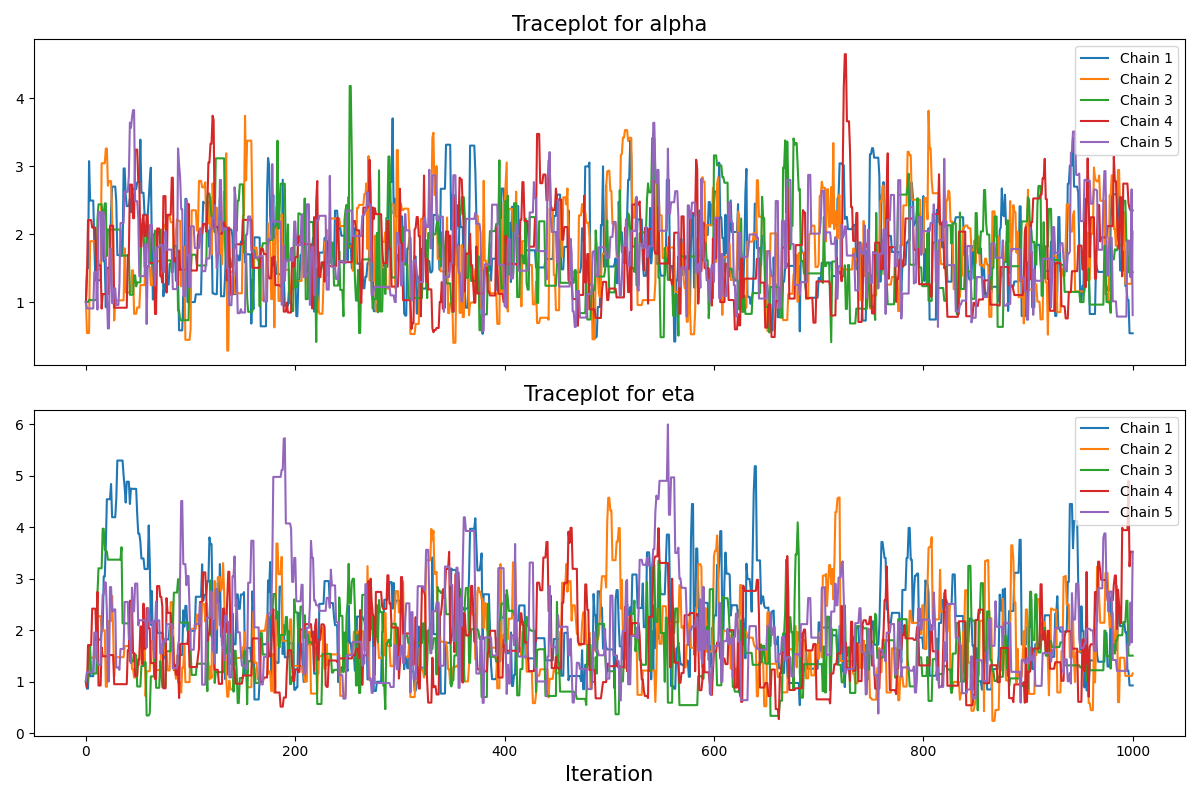
\includegraphics[width=0.99\columnwidth]{figures/mvn_trace.png}
        \caption{Trace plot for the multivariate normal proposal}
        \label{fig:mvn_trace}
    \end{figure}


        \begin{figure}[h]
        \centering
        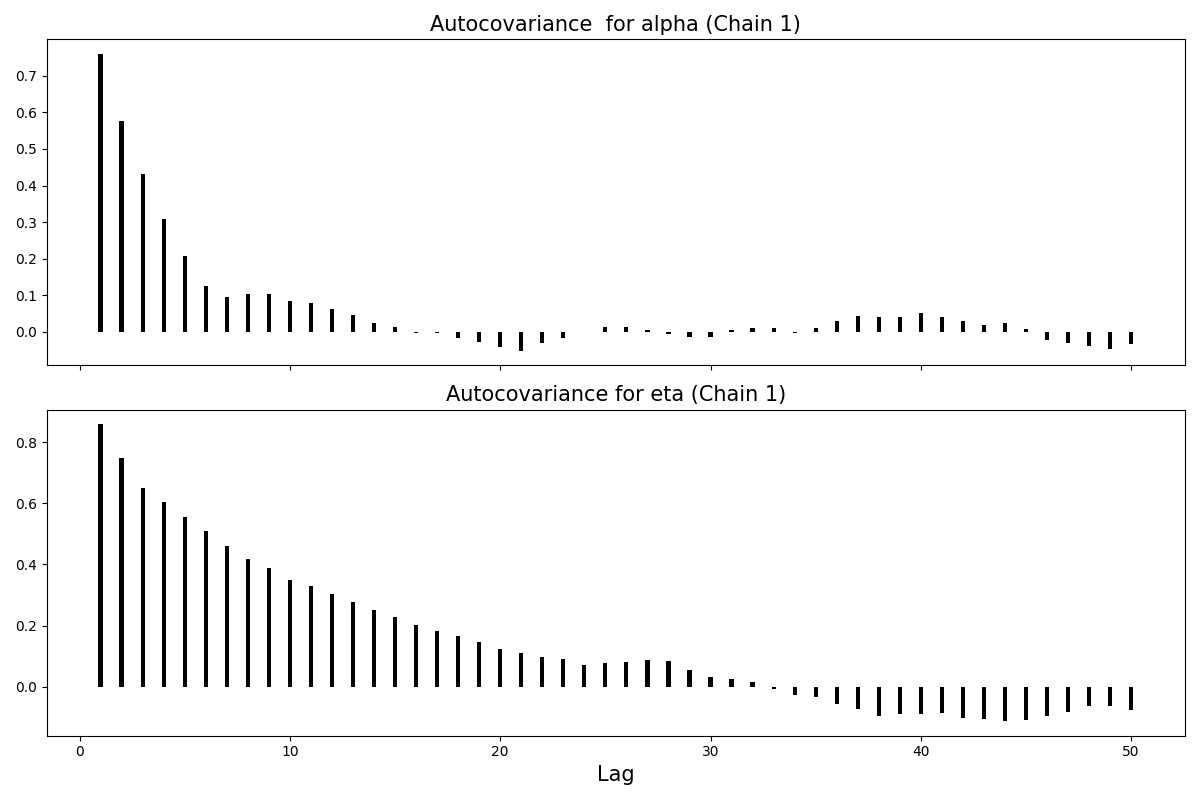
\includegraphics[width=0.99\columnwidth]{figures/mvn_cov.png}
        \caption{Autocovariance plot for the multivariate normal proposal}
        \label{fig:mvn_cov}
    \end{figure}


\subsection{The provided proposal}
Here we used: 
\[
q(\alpha', \eta' \mid \alpha, \eta) = \frac{1}{\alpha \eta} \exp\left( -\frac{\alpha'}{\alpha} - \frac{\eta'}{\eta} \right)
\]
as our proposal. This is a product of two exponential distributions, 
so we needed to sample like this:
\[
\alpha' \sim \text{Exp}(\lambda = 1/\alpha), \quad \eta' \sim \text{Exp}(\lambda = 1/\eta).
\]
Then with the chosen proposal, we calculated the overall mean and variance of the parameters across all chains:

\begin{itemize}
    \item $\alpha$: mean = 1.6501, variance = 0.5179
    \item $\eta$: mean = 1.8212, variance = 0.8255
\end{itemize} 

Next, we present the trace plot in Figure~\ref{fig:exp_trace}. It is evident that many proposals were rejected when using this exponential proposal distribution, as indicated by the flat segments in the traces. 

In contrast, the autocovariance plot in Figure~\ref{fig:exp_cov} shows that the autocovariance decreases slightly faster compared to the previous (normal) proposal distribution, suggesting improved mixing behavior.

Finally, we consider the Effective Sample Size (ESS) across all chains:
\begin{itemize}
    \item Total ESS for $\alpha$: 486.41
    \item Total ESS for $\eta$: 484.12
\end{itemize}

We can see that the ESS for both parameters is quite a lot higher in comparison to the multivariate 
normal distribution. 


    \begin{figure}[h]
        \centering
        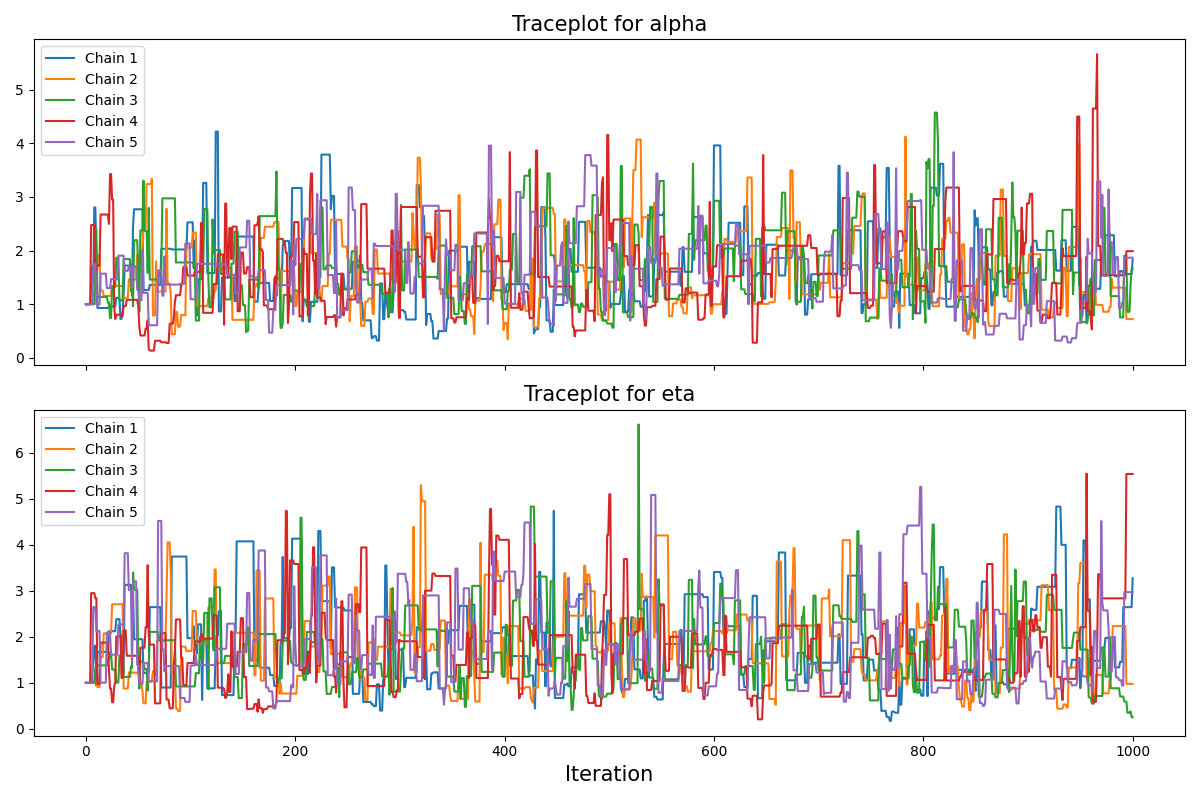
\includegraphics[width=0.99\columnwidth]{figures/exp_trace.png}
        \caption{Trace plot for the exponential proposal}
        \label{fig:exp_trace}
    \end{figure}


        \begin{figure}[h]
        \centering
        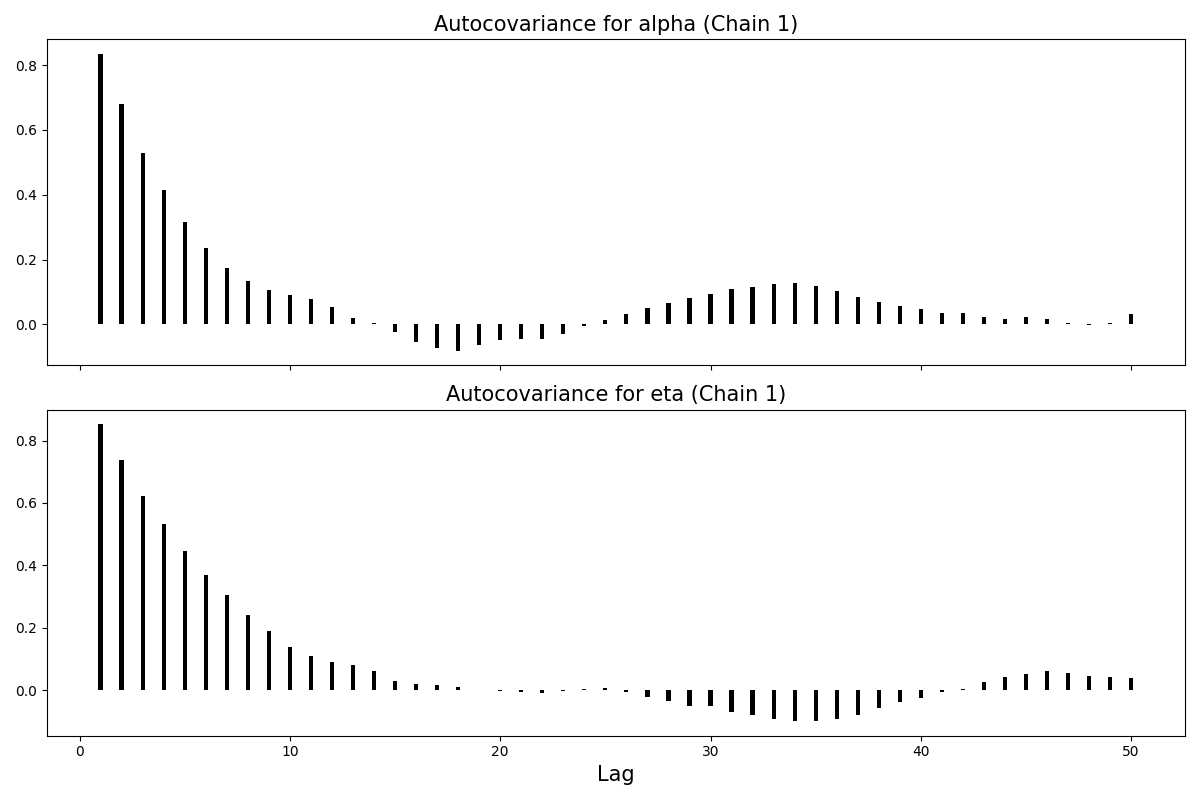
\includegraphics[width=0.99\columnwidth]{figures/exp_cov.png}
        \caption{Autocovariance plot for the exponential proposal}
        \label{fig:exp_cov}
    \end{figure}

\subsection{Comparison of both algorithms}

Based on the results, we observe that the Multivariate Normal proposal outperformed the 
Exponential proposal in terms of effective sample size and overall sampling efficiency. 
The MVN proposal yielded higher ESS values for both $\alpha$ and $\eta$, indicating better mixing 
and more informative samples across chains. However, achieving this performance required careful 
tuning of the proposal covariance matrix, which adds complexity and additional effort to the 
implementation. In contrast, the Exponential proposal, while slightly less efficient, 
had the advantage of not requiring such tuning, making it simpler and more straightforward to apply 
in practice.



\subsection{Probabilty estimation}
Lastly, we computed the probability \(P\big((\alpha, \eta) \in [1.3, \infty) \times [1.3, \infty)\big)\) using samples from both proposals. The estimated probabilities were:

\begin{itemize}
    \item Multivariate Normal proposal: \(\hat{P} = 0.5562\)
    \item Exponential proposal: \(\hat{P} = 0.4635\)
\end{itemize}

These results indicate that the multivariate normal proposal yields a higher estimated probability in the specified region compared to the exponential proposal.



\end{document}
